\documentclass[9pt,twocolumn]{opticajnl}
\journal{opticajournal}
\renewcommand*{\journalname}{Optics Letters}
\setboolean{shortarticle}{true}

% \title{Self-synchronized event-driven transmission hyperspectral imaging with multi-window time-warp compensation}
\title{A Self-Calibrated Neuromorphic Hyperspectral Imaging Framework}
\author[1]{Rongzhou}
\author[1]{Edmund Y. Lam}
\affil[1]{Department of Electrical and Electronic Engineering, The University of Hong Kong}
\dates{\today}
\ociscodes{(110.4234) Multispectral and hyperspectral imaging; (120.0120) Instrumentation, measurement, and metrology; (100.3010) Image reconstruction techniques; (110.1758) Computational imaging}
\doi{\url{}}

\begin{abstract}
We demonstrate a visible-band transmission hyperspectral system that drives a diffraction-scanned illumination across a specimen and records the induced intensity dynamics with an event camera. Instead of relying on calibrated motor encoders or trigger wiring, the method self-synchronizes the scan by analysing the event activity via auto- and self-cross-correlation, yielding forward/backward segmentation directly from the data stream. A piecewise-affine, multi-window time-warp model with soft spatial memberships then compensates acceleration-induced temporal shear by minimizing within-bin event variance, outperforming single-slope corrections under low-cost motor actuation. The reconstructed spectra match a reference hyperspectral camera even in low-light conditions where the frame-based sensor degrades, underlining the advantage of the event-driven capture. Planned benchmarks will quantify the performance of single-pass and multi-pass fusion under nominal and dimmed illumination.
\end{abstract}

\usepackage{ifthen}
\usepackage{placeins}
\usepackage{xcolor}
\usepackage{tikz}
\usetikzlibrary{arrows.meta,positioning}

% Yellow placeholder figure macro for drafts
\newcommand{\phfig}[2][0.95\linewidth]{%
  \begingroup\setlength{\fboxsep}{0pt}\colorbox{yellow!20}{%
    \parbox{#1}{\vspace{16mm}\centering\textbf{PLACEHOLDER}\\\small #2\vspace{14mm}}}%
  \endgroup}

\providecommand{\nocitefullrefs}[1]{}

\begin{document}

\maketitle

\section{Introduction}
Scanning hyperspectral imagers deliver high spectral resolution at the expense of mechanical complexity and strict synchronization between motion and detection elements~\cite{hagen2013review}. Conventional systems integrate encoder signals, tachometers, or trigger lines to maintain spatial--spectral registration, which complicates low-cost deployments and long-term stability~\cite{yeh2011selfcal,alhourani2023linescan}. Event cameras provide an alternative sensing modality: they asynchronously report logarithmic intensity changes with microsecond latency and high dynamic range, recording only the temporal variations induced by a spectral scan~\cite{gallego2020event}. Prior event-driven hyperspectral work has typically relied on actively modulated illumination or precisely calibrated scanning optics to ensure temporal alignment~\cite{reinbacher2016manifold,bardow2016simultaneous}. Here we pursue a self-synchronized architecture that accepts inexpensive, non-uniform motor motion and restores spectral structure algorithmically.

The system operates in transmission across the visible band (420--700~nm), reducing surface-scatter artefacts and enabling a tractable model that links event timing to wavelength. The key technical contributions are: (i) an event-domain auto-/self-cross-correlation strategy that segments forward and backward scans without auxiliary sensors; (ii) a multi-window, soft-membership time-warp compensation that minimizes within-bin variance to undo acceleration-induced temporal shear, extending piecewise-affine warps from event-motion studies~\cite{mitrokhin2018mobility}; and (iii) a reconstruction pipeline that integrates polarity-balanced events into spectral estimates, benchmarking them against a frame-based hyperspectral reference in both nominal and low-light regimes. Subsequent experiments will quantify the benefits of single-pass versus multi-pass fusion and assess robustness under reduced illumination, complementing the figure plan outlined below.

\section{System architecture and sensing model}
Figure~\ref{fig:overview}a sketches the optical layout. A broadband LED illuminates a specimen; a diffraction grating mounted in a 4$f$ relay is driven by a low-cost galvanometer or stepper stage to sweep the dispersed spectrum across a hybrid sensor plane that houses a dynamic vision sensor (DVS) and a co-aligned frame imager. The motor executes repeated forward/backward scans (currently three in each direction), but its speed is neither constant nor calibrated.

Under small-angle assumptions the wavelength incident on pixel $(x,y)$ is
\begin{equation}
  \lambda(x,t) \approx d\!\left(\frac{x}{z_2} - \frac{\xi(t)}{z_1}\right),
  \label{eq:lambda_mapping}
\end{equation}
where $d$ is the grating dispersion constant, $z_2$ and $z_1$ denote distances from the grating to the sensor and illumination relay, and $\xi(t)$ is the motor displacement inferred from the data stream. The transmitted intensity can be written as $I_{x,y}(t) = I_0^{(x,y)}[\lambda(x,t)]$, leading to the temporal gradient
\begin{equation}
  \frac{\partial I_{x,y}}{\partial t} = \frac{\partial I_0^{(x,y)}}{\partial \lambda} \frac{\partial \lambda(x,t)}{\partial t},
  \label{eq:intensity_gradient}
\end{equation}
which drives event emission when the logarithmic intensity crosses the sensor threshold. Because $\partial \lambda/\partial t$ is governed by the motor trajectory, reconstructing $I_0^{(x,y)}(\lambda)$ reduces to integrating polarity-weighted events along a synchronized wavelength axis.

\FloatBarrier
\begingroup\setlength{\abovecaptionskip}{2pt}\setlength{\belowcaptionskip}{0pt}
\begin{figure*}[!t]
  \centering
  \includegraphics[width=0.7\linewidth]{../../publication_code/figures/figure01_overview.pdf}
  \caption{System overview and modular integration. A dispersed illumination path (left, blue dashed box) acts as a drop-in module before the sample, while a non-intrusive detection add-on (right, green dashed box) uses a 4$f$ relay to feed an event+frame sensor. An optional splitter or camera port preserves the original microscope camera.}
  \label{fig:overview}
\end{figure*}
\endgroup

\section{Event-trigger probability model}
Event emission occurs when the logarithmic brightness increment surpasses a fixed magnitude $\theta$. Under realistic sensing conditions the observed gradient is corrupted by noise, which we model as
\begin{equation}
  \nabla I = \nabla I_{\text{true}} + \eta,\qquad \eta \sim \mathcal{N}(0,\sigma^2).
  \label{eq:gradient_noise}
\end{equation}
The probability of a positive event equals the likelihood that the noise-perturbed gradient exceeds the threshold,
\begin{equation}
  P(\text{event}) = P(\eta > \theta - \nabla I_{\text{true}}) = \tfrac12\!\left[1 - \operatorname{erf}\!\left(\frac{\theta - \nabla I_{\text{true}}}{\sqrt{2}\sigma}\right)\right],
  \label{eq:trigger_probability}
\end{equation}
with an analogous form for negative events around $-\theta$. Approximating the error function by a logistic curve yields the computationally convenient sigmoid expression
\begin{equation}
  P(\text{event}) \approx \sigma\!\left(\frac{\nabla I_{\text{true}} - \theta}{\sigma'}\right),\qquad \sigma' \approx \frac{2\sqrt{2}}{\sqrt{\pi}}\sigma,
  \label{eq:sigmoid_probability}
\end{equation}
where $\sigma(\cdot)$ denotes the logistic sigmoid. Within a temporal bin of duration $\Delta t$ the expected event count relates directly to this probability,
\begin{equation}
  \langle N_{\text{evt}}\rangle = \lambda\,P(\text{event})\,\Delta t,
  \label{eq:expected_events}
\end{equation}
with $\lambda$ the effective sampling rate per pixel. Averaging events over repeated scans gives the empirical mean $\bar{N}_{\text{evt}}$, which can be inverted via the logit function $\sigma^{-1}$ to estimate the true gradient:
\begin{equation}
  \nabla I_{\text{est}} = \theta + \sigma'\,\sigma^{-1}\!\left(\frac{\bar{N}_{\text{evt}}}{\lambda\,\Delta t}\right).
  \label{eq:gradient_estimate}
\end{equation}

This probabilistic link between event statistics and intensity gradients underpins our reconstruction strategy. Equation~(\ref{eq:gradient_estimate}) justifies using temporally binned events as sufficient statistics for spectral estimation: the scan-induced evolution of $\nabla I_{\text{true}}$ encodes spectral slopes, while averaging suppresses sensor noise and preserves the dynamic-range benefits of event vision. The next sections leverage these statistics to segment scans and correct the residual temporal shear before building the spectral cube.

\section{Self-synchronized scan segmentation}
We first convert the event timestamps into an activity signal $a[n]$ (events per 1~ms bin). A sliding window search identifies the densest subsequence containing at least 80\% of all events, yielding an initial round-trip estimate. The auto-correlation
\begin{equation}
  R[k] = \sum_{n} a[n]\,a[n+k]
\end{equation}
reveals the dominant period, while the reverse-correlation between $a[n]$ and $a[N{-}1{-}n]$ sharpens the turnaround index by exploiting mirror symmetry between forward and backward sweeps. An iterative peak search refines the start and end indices of each half-scan, producing six segments (three forward, three backward) without reference measurements. Anti-correlation further labels scan direction by comparing the sign of slope changes surrounding detected peaks.

This data-driven segmentation adapts to slow drifts or perturbations, ensuring that subsequent reconstructions operate on consistent temporal support. Planned experiments include (i) using only the first forward/back pair to quantify baseline noise, and (ii) averaging all three pairs to demonstrate variance reduction. Their results will populate Fig.~\ref{fig:segmentation}(d).

\begin{figure}[t]
  \centering
  \begin{tikzpicture}
    \node[anchor=south west, inner sep=0] (f2a) at (0,0)
      {\includegraphics[width=\linewidth]{../../publication_code/figures/figure02_activity.pdf}};
    \begin{scope}[x={(f2a.south east)}, y={(f2a.north west)}]
      \node[font=\bfseries, anchor=north west, fill=white, text=black, inner sep=2pt] at (0.012, 0.988) {(a)};
    \end{scope}
  \end{tikzpicture}\\[-2pt]
  \begin{tikzpicture}
    \node[anchor=south west, inner sep=0] (f2b) at (0,0)
      {\includegraphics[width=\linewidth]{../../publication_code/figures/figure02_correlation.pdf}};
    \begin{scope}[x={(f2b.south east)}, y={(f2b.north west)}]
      \node[font=\bfseries, anchor=north west, fill=white, text=black, inner sep=2pt] at (0.012, 0.988) {(b)};
    \end{scope}
  \end{tikzpicture}
  \vspace{-3pt}
  \caption{Self-synchronized scan segmentation. (a) Event activity over the full recording with pre-/post-scan shading and alternating forward/backward boundaries. (b) Auto- and reverse-correlation of the activity signal; the blue marker indicates the mirror-peak used to localize the turnaround.}
  \label{fig:segmentation}
\end{figure}

\section{Multi-window time-warp compensation}
Even with accurate segmentation, \eqref{eq:lambda_mapping} introduces a spatially varying delay through the $x/z_2$ term; motor acceleration near turnarounds further shears the time axis. Our multi-window compensation routine addresses this by fitting boundary surfaces
\begin{equation}
  T_i(x,y) = a_i x + b_i y + c_i,
\end{equation}
which partition each scan into $M$ temporal windows. Soft memberships,
\begin{equation}
  w_i(x,y,t) = \frac{\sigma\!\left(\frac{t - T_i}{\tau}\right)\sigma\!\left(\frac{T_{i+1}-t}{\tau}\right)}{\sum_j \sigma\!\left(\frac{t - T_j}{\tau}\right)\sigma\!\left(\frac{T_{j+1}-t}{\tau}\right)},
\end{equation}
blend adjacent windows (temperature $\tau \approx 1$~ms). The compensated time is
\begin{equation}
  t' = t - \sum_{i=1}^{M-1} w_i(x,y,t)\bigl(\tilde{a}_i x + \tilde{b}_i y \bigr),
  \label{eq:timewarp}
\end{equation}
where $\{\tilde{a}_i,\tilde{b}_i\}$ are optimized by minimizing the spatial variance of event counts within short $t'$ bins while penalizing abrupt parameter changes between neighbouring windows. Gradient-based updates use mini-batches of events to respect GPU memory limits. Compared with a single-plane warp (global $a,b$), the multi-window model better captures acceleration and deceleration phases, yielding sharper reconstructions.

Figure~\ref{fig:warp} will visualise diagnostics: (a) $x$--$t$ projections before compensation showing diagonal striations; (b) the same after applying \eqref{eq:timewarp}; (c) cumulative event frames before and after warping, highlighting blur reduction; and (d) the learned boundary curves $T_i(x)$ that reveal the motor’s velocity profile. Quantitative plots will report variance reductions and residual blur metrics contrasting the multi-window and single-plane models.

\begin{figure}[t]
  \centering
  % Figure 3(a): Events with learned boundaries (X--T and Y--T)
  \begin{tikzpicture}
    \node[anchor=south west, inner sep=0] (img3a) at (0,0)
      {\includegraphics[width=\linewidth]{../../publication_code/figures/figure03_a_events.pdf}};
    \begin{scope}[x={(img3a.south east)}, y={(img3a.north west)}]
      % Lift panel letter slightly above the image to avoid overlap
      \node[font=\bfseries, anchor=south west, fill=white, text=black, inner sep=2pt] at (0.010, 1.015) {(a)};
    \end{scope}
  \end{tikzpicture}\\[4pt]
  % Figure 3(b): Variance vs time (50 ms bins)
  \begin{tikzpicture}
    \node[anchor=south west, inner sep=0] (img3b) at (0,0)
      {\includegraphics[width=\linewidth]{../../publication_code/figures/figure03_b_variance.pdf}};
    \begin{scope}[x={(img3b.south east)}, y={(img3b.north west)}]
      % Lift panel letter slightly above the image to avoid overlap
      \node[font=\bfseries, anchor=south west, fill=white, text=black, inner sep=2pt] at (0.010, 1.015) {(b)};
    \end{scope}
  \end{tikzpicture}\\[4pt]
  % Figure 3(c): Single 50 ms bin comparison (original vs compensated)
  \begin{tikzpicture}
    \node[anchor=south west, inner sep=0] (img3c) at (0,0)
      {\includegraphics[width=\linewidth]{../../publication_code/figures/figure03_c_bin50ms.pdf}};
    \begin{scope}[x={(img3c.south east)}, y={(img3c.north west)}]
      % Lift panel letter slightly above the image to avoid overlap
      \node[font=\bfseries, anchor=south west, fill=white, text=black, inner sep=2pt] at (0.010, 1.015) {(c)};
    \end{scope}
  \end{tikzpicture}
  \caption{Multi-window compensation diagnostics. (a) X--T and Y--T event projections with the learned boundary surfaces overlaid (downsampled events; time normalized over the full scan for alignment). (b) Variance per 50~ms bin before and after compensation, showing reductions across most of the scan. (c) Example 50~ms bin illustrating visual improvement from original to compensated.}
  \label{fig:warp}
\end{figure}

\begin{figure*}[t]
  \centering
  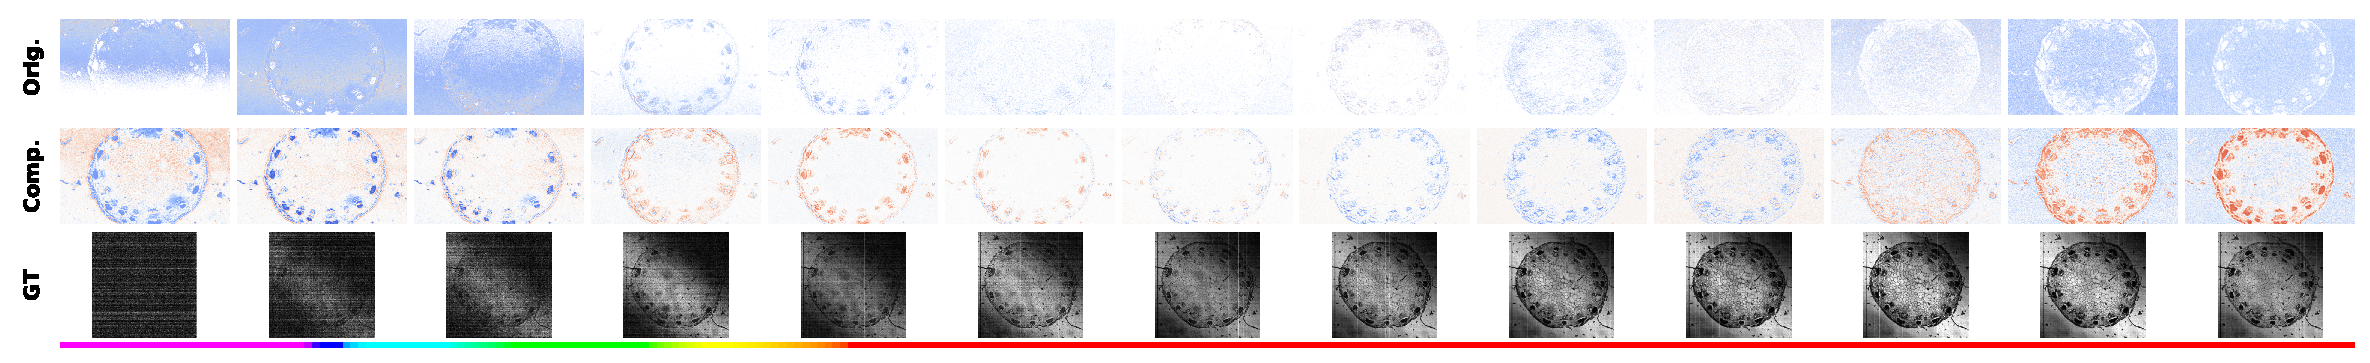
\includegraphics[width=0.98\textwidth]{../../publication_code/figures/figure04_allinone_20251101_161009/figure04_rescaled_grid_bins_03_15.pdf}
  \caption{Spectral reconstruction across a single forward scan. Each column shows a 50~ms temporal bin (top: original; bottom: compensated with 3$\times$3$\times$3 smoothing and background subtraction). The compensated row is annotated with the wavelength inferred from a flat-to-flat alignment of the 5~ms rescaled background spectrum to the spectrometer ground truth.}
  \label{fig:spectrum}
\end{figure*}

\section{Spectral reconstruction and benchmarking}
After compensation we bin events along $t'$ to obtain quasi-static frames $\mathsf{E}_k(x,y)$ over 1--2~ms intervals, integrate polarity-weighted counts to recover relative spectra, and optionally incorporate the frame camera as a DC reference. Three forward/backward cycles are currently fused to suppress noise, but the segmentation framework enables rigorous evaluation of single-cycle reconstructions. Ground-truth comparison uses a frame-based hyperspectral camera capturing the same scene; spectral overlays and residual maps quantify accuracy. Low-light trials---achieved by dimming the LED source---highlight the event camera’s high dynamic range: the reference system exhibits elevated noise and requires longer exposures, whereas the event reconstruction remains stable.

Figure~\ref{fig:spectrum} outlines the intended presentation: (a) reconstructed monochrome slices at representative wavelengths; (b) an RGB composite; (c) spectral curves comparing event reconstruction, reference camera, and residuals; and (d) a quantitative panel showing low-light error bars or forward-only versus multi-pass fusion performance. These visualisations will emphasise the system’s spectral fidelity and robustness in scenarios challenging for frame-based sensors.


\section{Discussion and outlook}
The self-synchronizing strategy removes the need for encoder calibration while tolerating speed fluctuations from cost-effective actuators, distinguishing this platform from prior systems that assumed precise timing hardware~\cite{hagen2013review,yeh2011selfcal}. The variance-minimizing, multi-window time warp extends piecewise-affine compensations used in event-based motion estimation~\cite{mitrokhin2018mobility}, adapting them to the spectral scanning context. Together these components enable transmission-mode spectral capture without illumination modulation or auxiliary sensors.

Next steps follow the planned figures: (i) gather datasets spanning single and triple scan fusion to populate Fig.~\ref{fig:segmentation}(d); (ii) quantify variance reduction and residual blur for multi-window versus single-plane warps to complete Fig.~\ref{fig:warp}; and (iii) collect spectral overlays under nominal and low-light scenarios to fill Fig.~\ref{fig:spectrum}. These experiments will cement the claims of self-synchronization, temporal correction, and low-light robustness.

\section{Conclusion}
We presented a self-synchronized, event-driven transmission hyperspectral system that derives scan timing from the event stream and compensates temporal shear using a multi-window time warp. Despite relying on inexpensive, non-uniform motor motion, the reconstructed spectra align with a reference hyperspectral camera and retain fidelity under reduced illumination. The mathematical framework and figure plan outlined here provide a clear roadmap toward a concise Optics Letters paper focused on the optical and computational innovation of event-based spectral acquisition.

\begin{thebibliography}{99}
\bibitem{hagen2013review} N. Hagen and M. Kudenov, ``Review of snapshot and scanning spectrometers,'' \emph{Opt. Eng.} \textbf{52}, 090901 (2013).
\bibitem{yeh2011selfcal} C.-K. Yeh and V. J. D. Tsai, ``Self-calibrated direct geo-referencing of airborne pushbroom hyperspectral images,'' in \emph{Proc. IGARSS}, 2881--2883 (2011).
\bibitem{alhourani2023linescan} A. Al-Hourani, M. F. Moghaddam, and N. Fassnacht, ``A line-scan hyperspectral imaging framework for low-cost deployments,'' \emph{Remote Sens.} \textbf{15}, 2787 (2023).
\bibitem{gallego2020event} G. Gallego, T. Delbrück, G. Orchard \emph{et~al.}, ``Event-based vision: A survey,'' \emph{IEEE Trans. Pattern Anal. Mach. Intell.} \textbf{44}, 154--180 (2022).
\bibitem{reinbacher2016manifold} C. Reinbacher, G. Graber, and T. Pock, ``Real-time intensity-image reconstruction for event cameras using manifold regularisation,'' in \emph{Proc. BMVC}, 1--12 (2016).
\bibitem{bardow2016simultaneous} P. Bardow, A. J. Davison, and S. Leutenegger, ``Simultaneous optical flow and intensity estimation from an event camera,'' in \emph{Proc. CVPR}, 884--892 (2016).
\bibitem{mitrokhin2018mobility} A. Mitrokhin, C. Fermüller, C. Parameshwara, and Y. Aloimonos, ``Event-based moving object detection and tracking,'' in \emph{Proc. ICRA}, 1--9 (2018).
\end{thebibliography}

\end{document}
